\documentclass[a4paper,12pt]{article}
\usepackage{etex}
%%%%%%%%%%%%%%%%%%%%%%%%%%%%%%%%%%%%%%
% Babel language package
\usepackage[english,greek]{babel}
% Inputenc font encoding
\usepackage[utf8]{inputenc}
%%%%%%%%%%%%%%%%%%%%%%%%%%%%%%%%%%%%%%

%%%%% math packages %%%%%%%%%%%%%%%%%%
\usepackage{amsmath}
\usepackage{amssymb}
\usepackage{amsfonts}
\usepackage{amsthm}
\usepackage{proof}

\usepackage{physics}

%%%%%%% symbols packages %%%%%%%%%%%%%%
\usepackage{dsfont}
\usepackage{stmaryrd}
%%%%%%%%%%%%%%%%%%%%%%%%%%%%%%%%%%%%%%%


%%%%%% graphicx %%%%%%%%%%%%%%%%%%%%%%%
\usepackage{graphicx}
\usepackage{color}
%\usepackage{xypic}
\usepackage[all]{xy}
\usepackage{calc}
%%%%%%%%%%%%%%%%%%%%%%%%%%%%%%%%%%%%%%%

\usepackage{enumerate}

\usepackage{fancyhdr}
%%%%% header and footer rule %%%%%%%%%
\setlength{\headheight}{14pt}
\renewcommand{\headrulewidth}{0pt}
\renewcommand{\footrulewidth}{0pt}
\fancypagestyle{plain}{\fancyhf{}
\fancyhead{}
\lfoot{}
\rfoot{\small \thepage}}
\fancypagestyle{vangelis}{\fancyhf{}
\rhead{\small \leftmark}
\lhead{\small }
\lfoot{}
\rfoot{\small \thepage}}
%%%%%%%%%%%%%%%%%%%%%%%%%%%%%%%%%%%%%%%

\usepackage{hyperref}
\usepackage{url}
%%%%%%% hyperref settings %%%%%%%%%%%%
\hypersetup{pdfpagemode=UseOutlines,hidelinks,
bookmarksopen=true,
pdfdisplaydoctitle=true,
pdfstartview=Fit,
unicode=true,
pdfpagelayout=OneColumn,
}
%%%%%%%%%%%%%%%%%%%%%%%%%%%%%%%%%%%%%%



\usepackage{geometry}
\geometry{left=25.63mm,right=25.63mm,top=36.25mm,bottom=36.25mm,footskip=24.16mm,headsep=24.16mm}

%\usepackage[explicit]{titlesec}
%%%%%% titlesec settings %%%%%%%%%%%%%
%\titleformat{\chapter}[block]{\LARGE\sc\bfseries}{\thechapter.}{1ex}{#1}
%\titlespacing*{\chapter}{0cm}{0cm}{36pt}[0ex]
%\titleformat{\section}[block]{\Large\bfseries}{\thesection.}{1ex}{#1}
%\titlespacing*{\section}{0cm}{34.56pt}{17.28pt}[0ex]
%\titleformat{\subsection}[block]{\large\bfseries{\thesubsection.}{1ex}{#1}
%\titlespacing*{\subsection}{0pt}{28.80pt}{14.40pt}[0ex]
%%%%%%%%%%%%%%%%%%%%%%%%%%%%%%%%%%%%%%

%%%%%%%%% My Theorems %%%%%%%%%%%%%%%%%%
\newtheorem{thm}{Θεώρημα}[section]
\newtheorem{cor}[thm]{Πόρισμα}
\newtheorem{lem}[thm]{λήμμα}
\theoremstyle{definition}
\newtheorem{dfn}{Ορισμός}[section]
\newtheorem{dfns}[dfn]{Ορισμοί}
\theoremstyle{remark}
\newtheorem{remark}{Παρατήρηση}[section]
\newtheorem{remarks}[remark]{Παρατηρήσεις}
%%%%%%%%%%%%%%%%%%%%%%%%%%%%%%%%%%%%%%%




\newcommand{\vect}[2]{(#1_1,\ldots, #1_#2)}
%%%%%%% nesting newcommands $$$$$$$$$$$$$$$$$$$
\newcommand{\function}[1]{\newcommand{\nvec}[2]{#1(##1_1,\ldots, ##1_##2)}}

\newcommand{\linode}[2]{#1_n(x)#2^{(n)}+#1_{n-1}(x)#2^{(n-1)}+\cdots +#1_0(x)#2=g(x)}

\newcommand{\vecoffun}[3]{#1_0(#2),\ldots ,#1_#3(#2)}



\input{insbox}

\linespread{1.2}

\pagestyle{askhseis}
\usepackage{cutwin}
\everymath{\displaystyle}

\begin{document}

\chapter{Ακρότατα Συναρτήσεων Πολλών Μεταβλητών}

\section{Τοπικά Ακρότατα}

\begin{dfn}
\item {}
  Έστω $ f \colon A \subseteq \mathbb{R}^{2} \to \mathbb{R} $, έστω 
  $ (x_{0}, y_{0}) \in A $ και έστω $R(x_{0}, y_{0}) $ περιοχή στοιχείων του $A$, 
  γύρω από το $ (x_{0}, y_{0}) $.
  \begin{enumerate}[i)]
    \item 
      Η $ f(x,y) $, έχει τοπικό ελάχιστο στο σημείο $ (x_{0}, y_{0}) $, αν 
      $ f(x_{0}, y_{0}) \leq f(x,y), \; \forall (x,y) \in R(x_{0}, y_{0}) $ 
    \item 
      Η $ f(x,y) $, έχει τοπικό μέγιστο στο σημείο $ (x_{0}, y_{0}) $, αν 
      $ f(x_{0}, y_{0}) \geq f(x,y), \; \forall (x,y) \in R(x_{0}, y_{0}) $ 
  \end{enumerate}
  Το τοπικά μέγιστο και το τοπικά ελάχιστο, ονομάζονται \textcolor{Col1}{τοπικά
  ακρότατα}. 
  Αν οι ανισότητες στον παραπάνω ορισμό, ισχύουν \textbf{για κάθε σημείο} στο πεδίο 
  ορισμού της συνάρτησης, τότε λέμε ότι η $f$ έχει \textcolor{Col1}{ολικό ακρότατο}.
\end{dfn}

\begin{prop}\label{prop:fermat2}
\item {}
  Αν η συνάρτηση $ f(x,y) $ έχει τοπικό ακρότατο στο σημείο $ (x_{0}, y_{0}) $, 
  τότε:
  \begin{enumerate}[i)]
    \item ή υπάρχουν οι $ f_{x}(x_{0}, y_{0}) $ και $ f_{y}(x_{0}, y_{0}) $ 
      και ισχύει $ f_{x}(x_{0}, y_{0}) = f_{y}(x_{0}, y_{0} )=0 $
    \item ή μία τουλάχιστον από τις $ f_{x}(x_{0}, y_{0}) $ και 
      $ f_{y}(x_{0}, y_{0}) $ δεν υπάρχει.
  \end{enumerate}
\end{prop}

\begin{rem}
\item {}
  Το αντίστροφο της παραπάνω πρότασης δεν ισχύει. 
\end{rem}

\begin{dfn}
  Τα \textbf{εσωτερικά} σημεία του πεδίου ορισμού της $ f(x,y) $, για τα οποία 
  υπάρχουν οι μερικές παράγωγοι 1ης τάξης, και είναι ίσες με 0 ή που δεν υπάρχει 
  τουλάχιστον μία εξ αυτών, λέγονται \textcolor{Col1}{κρίσιμα} ή
  \textcolor{Col1}{στάσιμα} σημεία της $ f(x,y) $. 
\end{dfn}

\begin{rem}
  Σύμφωνα με την πρόταση~\ref{prop:fermat2} τα \textbf{κρίσιμα} σημεία της $ f(x,y) $, 
  μαζί με τα \textbf{συνοριακά} σημεία του πεδίου ορισμού της (τα οποία είναι επίσης  
  σημεία όπου δεν ορίζονται οι μερικές παράγωγοι 1ης τάξης) είναι θέσεις \textbf{πιθανών} ακροτάτων.
\end{rem}

Όπως γνωρίζουμε για τις συναρτήσεις μιας μεταβλητής, ότι κάθε κρίσιμο σημείο δεν είναι 
αναγκαία τοπικό ακρότατο, γιατί μπορεί να είναι σημείο καμπής, έτσι κ για τις
συναρτήσεις δύο μεταβλητών, ένα κρίσιμο σημείο, μπορεί να είναι σαγματικό σημείο.

\begin{dfn}
  Ένα κρίσιμο σημείο $ (x_{0}, y_{0}) $, μιας διαφορίσιμης συνάρτησης $ f(x,y) $, είναι
  \textcolor{Col1}{σαγματικό σημείο}, αν για κάθε ανοιχτό δίσκο με κέντρο το 
  $ (x_{0}, y_{0}) $, υπάρχουν σημεία $ (x,y) $ στο πεδίο ορισμού της $f$, για τα 
  οποία, άλλοτε $ f(x,y) > f(x_{0}, y_{0}) $ κι άλλοτε $ f(x,y) < f(x_{0}, y_{0}) $. 
\end{dfn}

\begin{example}
\item {}
  \InsertBoxL{2}{\parbox[b][6\baselineskip][c]{0.28\textwidth}
  {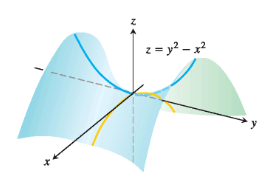
\includegraphics[scale=0.5]{saddle}}}
  Έστω η συνάρτηση $ f(x,y) = y^{2}-x^{2} $. Έχουμε ότι 
  $ f_{x}=-2x $ και $ f_{y}=2y $, άρα το $ (0,0) $ είναι το μοναδικό στάσιμο σημείο 
  της $f$. 
  Παρατηρούμε, ότι για όλα τα σημεία του άξονα $x$, άρα και για κάθε 
  $ (x,0) $ κοντά στο σημείο $(0,0)$, έχουμε ότι $ f(x,y) = -x^{2} < 0 $. 
  Όμως, για όλα τα σημεία του άξονα $ y $, άρα και για κάθε 
  $ (0,y) $ κοντά στο σημείο $ (0,0) $, έχουμε ότι $ f(x,y)=y^{2} > 0 $. 
  Άρα, σε κάθε 
  περιοχή του σημείου $ (0,0) $, πάντα θα βρίσκουμε τιμές της $ f(x,y) $ που είναι
  θετικές και αρνητικές. Άρα το σημείο $ (0,0) $ δεν μπορεί να είναι τοπικό ακρότατο 
  της $f$. Σε αυτή την περίπτωση, το σημείο $ (0,0) $ λέγεται \textbf{σαγματικό
  σημείο}, και μοιάζει με το σημείο στο κέντρο μιας σέλας, 
  όπως φαίνεται και στο σχήμα, γι᾽ αυτό και πολλές φορές χαρακτηρίζεται και ως 
  σελλοειδές σημείο.
\end{example}

\begin{dfn}
  Έστω $ (x_{0}, y_{0}) $ κρίσιμο σημείο της $f$. Ορίζουμε τις παρακάτω ορίζουσες:
  \[
    \abs{H_{1}} = f_{xx}(x_{0}, y_{0}) \quad \text{και} \quad 
    \abs{H_{2}} = \begin{vmatrix}
      f_{xx} & f_{xy} \\
      f_{yx} & f_{yy}
    \end{vmatrix}_{(x_{0}, y_{0})}
  \] 
\end{dfn}

\begin{thm}[Για συνάρτηση $ f(x,y) $ δύο μεταβλητών]
  \label{thm:2var}
\item {}
  Έστω $ f(x,y) $ συνάρτηση δύο μεταβλητών, ορισμένη σε ένα ανοιχτό 
  υποσύνολο $A$ του $ \mathbb{R}^{2} $, με μερικές παραγώγους 1ης και 2ης τάξης 
  ορισμένες σε μια  περιοχή του κρίσιμου σημείου $ (x_{0}, y_{0}) \in A $ και 
  έστω ότι οι παράγωγοι 2ης τάξης είναι συνεχείς στο $ (x_{0}, y_{0}) $. Τότε
\end{thm}

\begin{myitemize}
  \item Αν $ \abs{H_{1}} > 0 $ και $ \abs{H_{2}} > 0 $ τότε η $f$ παρουσιάζει στο 
    σημείο $ (x_{0}, y_{0}) $ \textbf{τοπικό ελάχιστο}.
  \item Αν $ \abs{H_{1}} < 0 $ και $ \abs{H_{2}} > 0 $ τότε η $f$ παρουσιάζει στο 
    σημείο $ (x_{0}, y_{0}) $ \textbf{τοπικό μέγιστο}.
  \item Αν $ \abs{H_{2}} < 0 $ τότε η $f$ δεν παρουσιάζει ακρότατο και σε αυτήν 
    την περίπτωση το σημείο λέγεται \textbf{σαγματικό}.
  \item Αν $ \abs{H_{2}} = 0 $, τότε δεν βγαίνει κάποιο συμπέρασμα σχετικά με το 
    σημείο $ (x_{0}, y_{0}) $.
\end{myitemize}

Το προηγούμενο θεώρημα επεκτείνεται και για συναρτήσεις με τρεις μεταβλητές. Σε αυτή 
την περίπτωση, εκτός από τις ορίζουσες $ \abs{H_{1}} $ και $ \abs{H_{2}} $, ορίζεται 
ακόμη η
\[
  \abs{H_{3}} = 
  \begin{vmatrix}
    f_{xx} & f_{xy} & f_{xz} \\
    f_{yx} & f_{yy} & f_{yz} \\
    f_{zx} & f_{zy} & f_{zz}
  \end{vmatrix} 
  \hfill 
\] 

\begin{rem}
  Όλες οι παραπάνω ορίζουσες ονομάζονται \textcolor{Col1}{Εσσιανές} και περιέχουν τις 
  παραγώγους 2ης τάξης της συνάρτησης. Οι αντίστοιχοι πίνακες, ονομάζονται 
  \textcolor{Col1}{Εσσιανοί} 
  και είναι \textbf{συμμετρικοί}, αφού από τις προϋποθέσεις του θεωρήματος ισχύει το 
  θεώρημα Schwartz και επομένως $ f_{xy} = f_{yx} $, $ f_{xz} = f_{zx} $, κλπ.
\end{rem}


\begin{thm}[Για συνάρτηση $ f(x,y,z) $ τριών μεταβλητών]
  \label{thm:3var}
\item {}
  Έστω $ f(x,y,z) $ συνάρτηση τριών μεταβλητών, ορισμένη σε ένα ανοιχτό 
  υποσύνολο $A$ του $ \mathbb{R}^{3} $, με μερικές παραγώγους 1ης και 2ης τάξης 
  ορισμένες σε μια  περιοχή του κρίσιμου σημείου $ (x_{0}, y_{0}, z_{0}) \in A $ και 
  έστω ότι οι παράγωγοι 2ης τάξης είναι συνεχείς στο $ (x_{0}, y_{0}, z_{0}) $. Τότε
\end{thm}

\begin{myitemize}
  \item Αν $ \abs{H_{1}} > 0 $, $ \abs{H_{2}} > 0 $ και $ \abs{H_{3}} > 0 $ 
    τότε η $f$ παρουσιάζει στο σημείο $ (x_{0}, y_{0}, z_{0}) $ \textbf{τοπικό ελάχιστο}.
  \item Αν $ \abs{H_{1}} < 0 $, $ \abs{H_{2}} > 0 $ και $ \abs{H_{3}} < 0 $ 
    τότε η $f$ παρουσιάζει στο σημείο $ (x_{0}, y_{0}, z_{0}) $ \textbf{τοπικό
    μέγιστο}.
  \item Αν $ \abs{H_{i}} \neq 0, \forall i \in \{1,2,3\} $ και δεν ισχύει κάποια 
    από τις προηγούμενες περιπτώσεις τότε η $f$ δεν παρουσιάζει ακρότατο και το 
    σημείο λέγεται \textbf{σαγματικό}.
  \item Αν μία τουλάχιστον από τις ορίζουσες $ \abs{H_{1}} $, $ \abs{H_{2}} $ και 
    $ \abs{H_{3}} $ είναι μηδέν, τότε δεν βγαίνει κάποιο συμπέρασμα σχετικά με το 
    σημείο $ (x_{0}, y_{0}, z_{0}) $.
\end{myitemize}

\section{Μεθοδολογία Εύρεσης τοπικών ακροτάτων για συνάρτηση δύο μεταβλητών}

\begin{enumerate}
  \item Βρίσκουμε όλες τις μερικές παραγώγους 1ης και 2ης τάξης.
  \item Βρίσκουμε τα κρίσιμα σημεία της συνάρτησης λύνοντας το σύστημα των εξισώσεων: 
    $ \begin{rcases}
      f_{x} = 0 \\
      f_{y} = 0  
    \end{rcases} $
  \item Για κάθε κρίσιμο σημείο, έστω $ (x_{0}, y_{0}), $ υπολογίζουμε τις Εσσιανές 
    ορίζουσες σε αυτό το σημείο και εφαρμόζουμε το θεώρημα~\ref{thm:2var}.
  \item Στην περίπτωση όπου $ \abs{H_{2}} = 0 $, τότε ακολουθούμε τον ορισμό των 
    τοπικών ακροτάτων.
    \begin{myitemize}
      \item Σχηματίζουμε τη διαφορά $ f(x,y) - f(x_{0}, y_{0}) $.
      \item Προσπαθούμε να προσδιορίσουμε το πρόσημό αυτής της διαφοράς σε 
        μια περιοχή του σημείου $ (x_{0}, y_{0}) $.
        \begin{myitemize}
          \item Αν $ f(x,y) - f(x_{0}, y_{0}) < 0, \; \forall (x,y) $ σε μια
            περιοχή του $ (x_{0}, y_{0}) $ τότε έχουμε ελάχιστο. 
          \item Αν $ f(x,y) - f(x_{0}, y_{0}) > 0, \; \forall (x,y) $ σε μια
            περιοχή του $ (x_{0}, y_{0}) $ τότε έχουμε μέγιστο. 
        \end{myitemize}
      \item Ειδικότερα, για να εξετάσουμε το σημείο $ (0,0) $ επιλέγουμε μια 
        καμπύλη που περνά από αυτό το σημείο, όπως για παράδειγμα 
        $ y= \lambda x $ ή $ y= \lambda x^{2} $, ώστε η διαφορά 
        $ f(x,y) - f(x_{0}, y_{0}) $ να εξαρτάται μόνο από το $x$ και να 
        είναι πιο εύκολο να προσδιορίσουμε το πρόσημό της.
    \end{myitemize}
\end{enumerate}

\section{Μεθοδολογία Εύρεσης τοπικών ακροτάτων για συνάρτηση τριών μεταβλητών}

\begin{enumerate}
  \item Βρίσκουμε όλες τις μερικές παραγώγους 1ης και 2ης τάξης.
  \item Βρίσκουμε τα κρίσιμα σημεία της συνάρτησης λύνοντας το σύστημα των εξισώσεων: 
    $ \begin{rcases}
      f_{x} = 0 \\
      f_{y} = 0 \\
      f_{z} = 0
    \end{rcases} $
  \item Για κάθε κρίσιμο σημείο, έστω $ (x_{0}, y_{0}, z_{0}), $ υπολογίζουμε 
    τις Εσσιανές ορίζουσες σε αυτό το σημείο και εφαρμόζουμε το 
    θεώρημα~\ref{thm:3var}.
  \item Στην περίπτωση όπου κάποια από τις ορίζουσες είναι μηδέν, τότε 
    ακολουθούμε τον ορισμό των τοπικών ακροτάτων.
    \begin{myitemize}
      \item Σχηματίζουμε τη διαφορά $ f(x,y,z) - f(x_{0}, y_{0}, z_{0}) $.
      \item Προσπαθούμε να προσδιορίσουμε το πρόσημό αυτής της διαφοράς σε 
        μια περιοχή του σημείου $ (x_{0}, y_{0}, z_{0}) $.
        \begin{myitemize}
          \item Αν $ f(x,y,z) - f(x_{0}, y_{0}, z_{0}) < 0, \; 
            \forall (x,y,z) $ σε μια
            περιοχή του $ (x_{0}, y_{0}, z_{0}) $ τότε έχουμε ελάχιστο. 
          \item Αν $ f(x,y,z) - f(x_{0}, y_{0}, z_{0}) > 0, \; 
            \forall (x,y,z) $ σε μια
            περιοχή του $ (x_{0}, y_{0}, z_{0}) $ τότε έχουμε μέγιστο. 
        \end{myitemize}
    \end{myitemize}
\end{enumerate}

Η γενίκευση του θεωρήματος τοπικών ακροτάτων για συναρτήσεις με περισσότερες 
μεταβλητές, γίνεται ως εξής: 

\begin{thm}
  Έστω $ f(x_{1},\ldots, x_{n}) $ συνάρτηση $n$ μεταβλητών, ορισμένη σε ένα ανοιχτό 
  υποσύνολο $A$ του $ \mathbb{R}^{n} $, με μερικές παραγώγους 1ης και 2ης τάξης 
  ορισμένες σε μια  περιοχή του κρίσιμου σημείου $P_{0}$ και έστω ότι οι παράγωγοι 
  2ης τάξης είναι συνεχείς στο $P_{0}$. Τότε, αν $ a_{ij} =
  \eval{\pdv[2]{f}{i}{j}}_{P_{0}}, 
  \forall i,j = 1,\ldots, n$, ορίζουμε τις 
  \[
    \abs{H_{1}} = a_{11}, \quad 
    \abs{H_{2}} = 
    \begin{vmatrix}
      a_{11} & a_{12} \\
      a_{21} & a_{22}
    \end{vmatrix}, \quad \ldots \quad 
    \abs{H_{n}} = 
    \begin{vmatrix}
      a_{11} & a_{12} & \cdots & a_{1n} \\
      a_{21} & a_{22} & \cdots & a_{2n} \\
      \vdots & \vdots & \cdots & \vdots \\
      a_{n1} & a_{n2} & \cdots & a_{nn} \\
    \end{vmatrix} 
  \]
  Τότε:

  \begin{myitemize}
    \item Αν $ \abs{H_{1}} >0 $, $ \abs{H_{2}} >0, \ldots, \abs{H_{n}} > 0 $, 
      τότε η $f$ παρουσιάζει στο $ P_{0} $ τοπικό ελάχιστο.
    \item Αν $ \abs{H_{1}} <0 $, $ \abs{H_{2}} >0, \ldots, 
      (-1)^{n}\abs{H_{n}} > 0 $, τότε η $f$ παρουσιάζει στο $ P_{0} $ τοπικό 
      μέγιστο.
    \item Αν $ \abs{H_{i}} \neq 0, \forall i \in \{1,\ldots,n\} $ και δεν ισχύει 
      κάποια από τις προηγούμενες περιπτώσεις τότε η $f$ δεν παρουσιάζει 
      ακρότατο και το σημείο λέγεται σαγματικό.
    \item Αν μία τουλάχιστον από τις ορίζουσες $ \abs{H_{1}}, \ldots, \abs{H_{3}} $ 
      είναι μηδέν, τότε δεν βγαίνει κάποιο συμπέρασμα σχετικά με το 
      σημείο $P_{0} $.
  \end{myitemize}
\end{thm}

\begin{rem}
  Ένας σύντομος μνημονικός κανόνας για τα ακρότατα των συναρτήσεων πολλών μεταβλητών, 
  είναι ο εξής:
  \begin{myitemize}
    \item Αν όλες οι Εσσιανές ορίζουσες είναι θετικές στο $ P_{0} $, τότε η 
      $f$ παρουσιάζει τοπικό ελάχιστο.
    \item Αν οι Εσσιανές ορίζουσες, έχουν πρόσημα εναλλάξ στο $ P_{0} $, με 
      την πρώτη να είναι αρνητική, τότε η $f$ παρουσιάζει τοπικό μέγιστο.
  \end{myitemize}
\end{rem}

\section{Ολικά Ακρότατα}

Ένα υποσύνολο $D$ του $ \mathbb{R}^{2} $ ονομάζεται \textcolor{Col1}{κλειστό}, αν 
περιέχει και όλα τα συνοριακά του σημεία, ενώ ονομάζεται \textcolor{Col1}{φραγμένο}, αν 
υπάρχει δίσκος του $ \mathbb{R}^{2} $ που το περιέχει, δηλαδή, ουσιαστικά ότι είναι 
περιορισμένο σε έκταση.

\begin{thm}
  Αν $f(x,y)$ είναι συνεχής σε κάποιο \textbf{κλειστό} και \textbf{φραγμένο} υποσύνολο 
  $A$ του $ \mathbb{R}^{2} $, τότε η $f$ παίρνει μέγιστη και ελάχιστη τιμή στο $A$. 
  Δηλαδή, υπάρχουν σημεία $ (x_{1}, y_{1}) \in A $ και $ (x_{2}, y_{2}) \in A $ τέτοια 
  ώστε 
  \[
    f(x_{1}, y_{1}) \leq f(x,y) \leq f(x_{2}, y_{2}), \quad \forall (x,y) \in A
  \]
\end{thm}

Η μέγιστη και η ελάχιστη τιμή του προηγούμενου θεωρήματος, είναι το \textbf{ολικά
ακρότατα} της συνάρτησης, και για να τα προσδιορίσουμε ακολουθούμε τα παρακάτω βήματα.

\begin{myitemize}
  \item Βρίσκουμε τις τιμές των κρίσιμων σημείων της $f$ στο $A$.
  \item Βρίσκουμε τις τιμές των τοπικών ακροτάτων της $f$ στο σύνορο του $A$. 
  \item Η μεγαλύτερη από τις τιμές που βρήκαμε στα πρώτα δύο βήματα 
    είναι το ολικό μέγιστο της συνάρτησης, ενώ η μικρότερη είναι το ολικό ελάχιστο.
\end{myitemize}




\chapter{Ακρότατα Υπό Συνθήκη}

\section{Πολλαπλασιαστές Lagrange}

\subsection{Ακρότατα υπό μία συνθήκη}

\enlargethispage{2\baselineskip}

\begin{thm}
  Έστω $ f(x,y) $ συνάρτηση δύο μεταβλητών, ορισμένη σε ένα ανοιχτό 
  υποσύνολο $A$ του $ \mathbb{R}^{2} $ και έστω ότι οι παράγωγοι 2ης τάξης είναι 
  συνεχείς στο $A$. Υποθέτουμε ότι για την συνάρτηση $ \phi $ οι μερικές παράγωγοι 
  1ης τάξης είναι συνεχείς στο $A$ και ικανοποιείται η συνθήκη 
  \begin{equation}
    \label{eq:constr1}
    \phi (x,y) = 0
  \end{equation}
  Θεωρούμε τη συνάρτηση Lagrange που ορίζεται από τον τύπο
  \[
    L(x,y, \lambda) = f(x,y) + \lambda \phi (x,y) 
  \] 
  και την ορίζουσα
  \[
    % \abs{\overline{H}_{1}} = 
    % \begin{vmatrix}
    %   L_{xx} & L_{xy} & L_{xz} & {\phi}_{x} \\
    %   L_{yx} & L_{yy} & L_{yz} & {\phi}_{y} \\
    %   L_{zx} & L_{zy} & L_{zz} & {\phi}_{z} \\
    %   {\phi}_{x} & {\phi}_{y} & {\phi}_{z} & 0
    % \end{vmatrix}, \quad 
    \abs{\overline{H}_{2}} = 
    \begin{vmatrix}
      L_{xx} & L_{xy} & \phi(x) \\
      L_{yx} & L_{yy} & \phi(y) \\
      \phi(x) & \phi(y) & 0
    \end{vmatrix}, \quad 
  \] 
  Υποθέτουμε ότι $ (x_{0}, y_{0}, \lambda) $ είναι μια λύση του συστήματος 
  \[
    \left.
      \begin{matrix}
        L_{x} = 0 \\
        L_{y} = 0 \\
        L_{\lambda} = 0 \\
      \end{matrix}
    \right\} 
  \]
  Τότε:
  \begin{myitemize}
    \item Αν $ \abs{\overline{H}_{2}} < 0 $ στο σημείο $ (x_{0}, y_{0}, \lambda) $, 
      τότε η $f$ παρουσιάζει \textbf{τοπικό ελάχιστο} στο $ (x_{0}, y_{0}) $ υπό τη
      συνθήκη του περιορισμού~\eqref{eq:constr1}.
    \item Αν $ \abs{\overline{H}_{2}} > 0 $ στο σημείο $ (x_{0}, y_{0}, \lambda) $, 
      τότε η $f$ παρουσιάζει \textbf{τοπικό μέγιστο} στο $ (x_{0}, y_{0}) $ υπό τη
      συνθήκη του περιορισμού~\eqref{eq:constr1}.
    \item Αν $ \abs{H_{2}} = 0 $, τότε δεν βγαίνει κάποιο συμπέρασμα σχετικά με το 
      σημείο $ (x_{0}, y_{0}) $.
  \end{myitemize}
\end{thm}

\begin{thm}
  Έστω μια συνάρτηση δύο μεταβλητών $ f(x,y) $ με τον περιορισμό $ \phi (x,y) = 0 $. 
  Θεωρούμε τη συνάρτηση Lagrange 
  \[
    L(x,y) = f(x,y) + \lambda \phi (x,y) 
  \]
  Τα ακρότατα $ P(x,y) $ της συνάρτησης $ f(x,y) $ υπό τον περιορισμό $ \phi (x,y)=0 $  
  θα αναζητηθούν από την λύση του συστήματος 
  \[
    \left.
      \begin{matrix}
        \grad L(x,y)=0 \\
        \phi (x,y)=0
      \end{matrix} 
    \right\} 
  \]
  Το σημείο $ P(x,y) $ θα είναι: 
  \begin{myitemize}
    \item \textbf{τοπικό ελάχιστο} αν $ [H(L(P)) \mathbf{u}] \cdot \mathbf{u} > 0 $
    \item \textbf{τοπικό μέγιστο} αν $ [H(L(P)) \mathbf{u}] \cdot \mathbf{u} < 0 $
  \end{myitemize}
\end{thm}
όπου $ H(L(P)) $ είναι η \textbf{Εσσιανή} ορίζουσα της συνάρτησης Lagrange στο 
σημείο $P$ και $ \mathbf{u} $ ένα οποιοδήποτε διάνυσμα \textbf{κάθετο} στο διάνυσμα της 
κλίσης της συνάρτησης $ \phi(x,y) $.


\end{document}
